\chapter{Experiments}\label{chap:experiments}
In this section we will test the methods discussed in \ref{sec:second}, and evaluate their performance for different models. We want to investigate whether the methods presented in the previous sections actually perform better in a tall data situation than the regular MH algorithm.  \\
The methods we have tested are given in the table below: 

\begin{table}[H]
    \centering
        \begin{tabular}{|c|c|c|c|c|}
    \hline
    \multicolumn{5}{|c|}{Methods} \\
    \hline
   Model & MH & FlyMC & Bardenet et. al 2014 & Bardenet et al. 2017\\ \hline\hline
        Gaussian & V & V & V &V \\
        Logistic regression &V &V &V &V  \\
        Linear regression &V & V& X& X \\ \hline
    \end{tabular}{}
    \caption{Overview of which models we have tested for the different methods. Here V indicates that the model is tested, and X that it is not.}
    \label{tab:experiment_overview}
\end{table}{}
We will use the number of required likelihood evaluations before convergence of the chain to the invariant distribution to be a measure of a methods performance.
Here, we will use the Gelman-Rubin statistic as a criterion for convergence, and also use the within chain correlation and other criteria to assess the quality of the method. 
\todo{fiks setning}
\texttt{Obviously} the methods presented in the previous sections have fewer likelihood evaluations per iteration, but one can imagine that because of fewer likelihood evaluations, the number of iterations needed to mixing may be larger than for the vanilla MH algorithm. 


\section{Logistic regression}\label{subsec:data}
In this thesis, we will test different methods for \textbf{statistical inference} on simulated binary data. These data are simulated in R in the following way
\begin{lstlisting}[caption={simulation of binary data}, label={lst:simulation}]
set.seed(23423)
n = 1000
x = sort(rnorm(n))
beta = c(1,2)
logist = function(x){1/(1+exp(-x))}
p = logist(beta[1]+beta[2]*x)
y = rbinom(n,1,prob=p)
\end{lstlisting}
\begin{figure}
    \centering
    \includegraphics[width=\textwidth]{example-image-a}
    \caption{Histogram over simulated data}
    \label{fig:my_label}
\end{figure}{}

As we see from listing \ref{lst:simulation}, we first draw standard normal data $x$, and define $\beta_1 = 1, \beta_2 = 2$. Next, we plug the  $u = \beta_1 + \beta_2 x$ into the logistic cumulative density. 
This results in a vector of probabilities, which we use to draw binary data $y$. Although this is a very simple method for data generation, if we are to perform logistic regression on the data $x$, and the response $y$ using MCMC methods, this may run slowly on a computer if there is a lot of data.


\section{Standard normal data}
We simulated standard normal data as shown below and used the different MCMC methods discussed in the methods section to make inference about the model parameters. 
\begin{lstlisting}[caption={simulation of standard normal data}, label={lst:sim_normal}]
set.seed(1234)
N = 1000
x = rnorm(N, 0, 1)
\end{lstlisting}
In this experiment, we have sampled $\sigma$ on a log-scale, and adjusted the proposal distribution accordingly. 
\subsection{Table of likelihood evaluations}
\begin{table}
    \centering
\begin{tabular}{|c|c|c|c|c|}
  \hline
    \multicolumn{5}{|c|}{10 000 MCMC iterations} \\
    \hline
\hline
        $\theta_{init}$ &  MH & FlyMC & Bardenet et al. 2014 & Bardenet et al. 2017\\ 
         \hline \hline$\theta_1$ & $20,000,000$ & $1,180,744$ & $11,317,284$ & $17,577,360$ \\
        $\theta_2$ & $20,000,000$ & $1,181,456$ & $11,491,240$ & $17,671,728$ \\
        $\theta_3$ & $20,000,000$ & $1,223,534$ & $11,426,232$ & $17,734,040$
        \\ $ \theta_4$ & $20,000,000$ & $1,168,024$ & $11,466,964$ & $17,682,160$ \\
        $\theta_5$ &$20,000,000$&$1,341,116$&$11,355,248$&$17,694,600$
        \\ \hline
\end{tabular}
\caption{The number of likelihood evaluations for each method with different starting values for $\theta$, with 10000 MCMC iterations.}
\label{tab:ll_evals_10k_normal}
\end{table} 

 \begin{table}
    \centering
\begin{tabular}{|c|c|c|c|c|}
  \hline
    \multicolumn{5}{|c|}{50 000 MCMC iterations} \\
    \hline
\hline
        $\theta_{init}$ &  MH & FlyMC & Bardenet et al. 2014 & Bardenet et al. 2017\\ 
         \hline \hline$\theta_1$ & $100,000,000$ & $5,916,530$ & $56,730,732$ & $87,796,872$ \\
        $\theta_2$ & $100,000,000$ & $5,945,652$ & $57,139,170$ & $88,133,312$ \\
        $\theta_3$ & $100,000,000$ & $6,259,376$ & $57,046,292$ & $88,060,816$
        \\ $ \theta_4$ & $100,000,000$ & $5,968,036$ & $57,396,190$ & $88,058,408$ \\
        $\theta_5$ &$100,000,000$&$6,468,548$&$57,097,776$&$88,292,392$
        \\ \hline
\end{tabular}
\caption{The number of likelihood evaluations for each method with different starting values for $\theta$ with 50000 MCMC iterations.}
\label{tab:ll_evals_50k_normal}
\end{table} 

 \begin{table}
    \centering
\begin{tabular}{|c|c|c|c|c|}
  \hline
    \multicolumn{5}{|c|}{100 000 MCMC iterations} \\
    \hline
\hline
        $\theta_{init}$ &  MH & FlyMC & Bardenet et al. 2014 & Bardenet et al. 2017\\ 
         \hline \hline$\theta_1$ & $200,000,000$ & $12,203,876$ & $113,786,516$ & $176,457,944$ \\
        $\theta_2$ & $200,000,000$ & $11,994,984$ & $113,961,610$ & $175,813,952$ \\
        $ \theta_3$ & $200,000,000$ & $11,862,396$ & $114,699,276$ & $176,127,488$ \\
        $\theta_4$ & $200,000,000$ & $12,680,344$ & $114,265,162$ & $176,973,752$ \\
        $\theta_5$ &$2000,000,000$&$11,653,048$&$114,328,384$&$176,256,160$
        \\ \hline
\end{tabular}
\caption{The number of likelihood evaluations for each method with different starting values for $\theta$ with 100 000 MCMC iterations.}
\label{tab:ll_evals_100k_normal}
\end{table} 
\subsection{Plot for 10k iterations}
\begin{figure}%
    \centering
    \subfloat[$\theta_{init} = \theta_1$]{\includegraphics[scale=0.3, page = 2]{figures/Normal/10k_04_06_theta1.pdf}}%
    \qquad
    \subfloat[$\theta_{init} = \theta_2$]{\includegraphics[scale=0.3, page = 2]{figures/Normal/10k_04_06_theta2.pdf}}%
    \newline
    \subfloat[$\theta_{init} = \theta_3$]{\includegraphics[scale=0.3, page = 2]{figures/Normal/10k_04_06_theta3.pdf}}%
    \qquad
    \subfloat[$\theta_{init} = \theta_4$]{\includegraphics[scale=0.3, page = 2]{figures/Normal/10k_04_06_theta4.pdf}}%
    \newline
     \subfloat[$\theta_{init} = \theta_5$]{\includegraphics[scale=0.3, page = 2]{figures/Normal/10k_04_06_theta5.pdf}}%
    \caption{Estimated posterior densities for all methods, with different starting values for $\theta$. The model is the normal distribution with parameters $\mu$ and $\sigma$, with $\sigma$ plotted on log-scale.}%
    \label{fig:density_10k_04_06_normal}%
\end{figure}




\begin{figure}%

    \caption{Autocorrelation for all methods, with different starting values for $\theta$. }%
      \centering
    \subfloat[$\theta_{init} = \theta_1$]{\includegraphics[scale=0.3, page = 6]{figures/Normal/10k_04_06_theta1.pdf}}%
    \qquad
    \subfloat[$\theta_{init} = \theta_2$]{\includegraphics[scale=0.3, page = 6]{figures/Normal/10k_04_06_theta2.pdf}}%
    \newline
    \subfloat[$\theta_{init} = \theta_3$]{\includegraphics[scale=0.3, page = 6]{figures/Normal/10k_04_06_theta3.pdf}}%
    \qquad
    \subfloat[$\theta_{init} = \theta_4$]{\includegraphics[scale=0.3, page = 6]{figures/Normal/10k_04_06_theta4.pdf}}%
    \newline
     \subfloat[$\theta_{init} = \theta_5$]{\includegraphics[scale=0.3, page = 6]{figures/Normal/10k_04_06_theta5.pdf}}%
    \label{fig:autocorrelation_10k_04_06_normal}%
\end{figure}

\subsection{Plot for 50k iterations}
\begin{figure}%
    \centering
    \subfloat[$\theta_{init} = \theta_1$]{\includegraphics[scale=0.3, page = 2]{figures/Normal/50k_04_06_theta1.pdf}}%
    \qquad
    \subfloat[$\theta_{init} = \theta_2$]{\includegraphics[scale=0.3, page = 2]{figures/Normal/50k_04_06_theta2.pdf}}%
    \newline
    \subfloat[$\theta_{init} = \theta_3$]{\includegraphics[scale=0.3, page = 2]{figures/Normal/50k_04_06_theta3.pdf}}%
    \qquad
    \subfloat[$\theta_{init} = \theta_4$]{\includegraphics[scale=0.3, page = 2]{figures/Normal/50k_04_06_theta4.pdf}}%
    \newline
     \subfloat[$\theta_{init} = \theta_5$]{\includegraphics[scale=0.3, page = 2]{figures/Normal/50k_04_06_theta5.pdf}}%
    \caption{Estimated posterior densities for all methods, with different starting values for $\theta$.  }%
    \label{fig:density_50k_04_06_normal}%
\end{figure}




\begin{figure}%

    \caption{Autocorrelation for all methods, with different starting values for $\theta$. }%
      \centering
    \subfloat[$\theta_{init} = \theta_1$]{\includegraphics[scale=0.3, page = 6]{figures/Normal/50k_04_06_theta1.pdf}}%
    \qquad
    \subfloat[$\theta_{init} = \theta_2$]{\includegraphics[scale=0.3, page = 6]{figures/Normal/50k_04_06_theta2.pdf}}%
    \newline
    \subfloat[$\theta_{init} = \theta_3$]{\includegraphics[scale=0.3, page = 6]{figures/Normal/50k_04_06_theta3.pdf}}%
    \qquad
    \subfloat[$\theta_{init} = \theta_4$]{\includegraphics[scale=0.3, page = 6]{figures/Normal/50k_04_06_theta4.pdf}}%
    \newline
     \subfloat[$\theta_{init} = \theta_5$]{\includegraphics[scale=0.3, page = 6]{figures/Normal/50k_04_06_theta5.pdf}}%
    \label{fig:autocorrelation_50k_04_06_normal}%
\end{figure}

\begin{figure}%
    \centering
    \subfloat[A]{\includegraphics[scale=0.3, page = 3]{figures/Normal/naive_compared1.pdf}}%
    \qquad
    \subfloat[B]{\includegraphics[scale=0.3, page = 3]{figures/Normal/flyMC_compared1.pdf}}%
    \newline
    \subfloat[C]{\includegraphics[scale=0.3, page = 3]{figures/Normal/confidence_compared1.pdf}}%
    \qquad
    \subfloat[D]{\includegraphics[scale=0.3, page = 3]{figures/Normal/confidence_w_pr_compared1.pdf}}%
    \caption{All plots A-D shows a Metropolis-Hastings chain, chain 1, plotted together with one other method. In Figure \ref{fig:compare_theta1}.A, chain 2 is the naive subsampler. In Figure\ref{fig:compare_theta1}.B, chain 2 is the Firefly, Figure \ref{fig:compare_theta1}.C is the Bardenet et al. 2014 subsampler and Figure \ref{fig:compare_theta1}.D is the Bardenet et al. 2017 subsampler. $\theta
   ^{\left(0\right)} ig:= \left(-0.2, -0.05\right)$}%
    \label{fig:compare_theta1_normal}%
\end{figure}


\subsection*{Metropolis-Hastings}\label{subsec:mh_sim}
\subsubsection{10k iterations}
We ran five chains with different starting values $\theta_{\texttt{init}}$ for $\theta = \left(\mu, \sigma\right)$, where $\theta_{\texttt{init}} \sim \mathcal{N}\left(\theta_{ML}, \; 0.1\right)$. 
\
Looking at Figure , we see that the chain seems to behave nicely. If we look closely, we can see that some of the starting values may be a bit off, but that this stabilizes quite quickly. We can confirm that the chain $\textbf{mixes nicely}$ by looking at the running average of the simulated $\textbf{parameters}$.
\
We will also look at the autocorrelation of the chains, also known as the within chain correlation. 

From Figure , we see that there is a lot of correlation in the early stages of the simulation, but that this decreases when the number of iterations is increased. After $10000$ iterations the adjusted Gelman-Rubin statistic, $\hat{R}$, given by \eqref{eq:Gelman-Rubin_adjusted},\textbf{Sett inn Gelman-Rubin verdier her}

Compared to the simulations from the Metropolis-Hastings algorithm, we see from Figure \ref{fig:simval_fly}, that the number of iterations needed before \textbf{convergence} is quite large. 


\subsection{Bardenet et al.'s confidence sampler}

\subsection{Firefly Monte Carlo}
The experiment design for the Firefly Monte Carlo simulation was the same as described in \ref{subsec:mh_sim}. The exactly the same $\theta_{\texttt{init}}$ where used in these simulations as in the case of the Metropolis-Hastings simulations. 

Compared to the simulations from the Metropolis-Hastings algorithm, we see from Figure \ref{fig:simval_fly}, that the number of iterations needed before \textbf{convergence} is quite large. 



\subsection{Bardenet et al.'s confidence sampler}





\subsection{Bardenet et al.'s confidence sampler with proxy}






\section*{Results}
We have implemented the Firefly Monte Carlo method, and tried logistic regression on simulated data, as described in section \ref{subsec:data} using both a regular MH-sampler as well as the Firefly Monte Carlo. 
We have also tried logistic regression on two of the classes \textbf{which classes} from MNIST data set \textbf{reference} where we calculate the principal components and use these as explanatory variables for the regression, as demonstrated in \cite{Maclaurin:1}. 

\subsection{Confidence sampler with proxy}
As we saw in \ref{sec:adap_subsampl}, we need a proxy $\powerset_i\left(\theta, \theta'\right)$ with $$\powerset_i\left(\theta, \theta'\right) \approx \ell_i\left(\theta'\right) - \ell_i\left(\theta\right). $$   
We will use a second order Taylor expansion as the proxy, i.e 
\begin{equation}
    \powerset_i\left(\theta, \theta'\right) = \hat{\ell}_i\left(\theta'\right) - \hat{\ell}_i\left(\theta\right) \approx \ell_i\left(\theta'\right) - \ell_i\left(\theta\right)
\end{equation}
with $\hat{\ell}_i\left(\theta\right)$ the second order Taylor expansion of $\ell_i\left(\theta\right)$, where the Taylor expansion of $\ell_i\left(\theta\right)$ is presented in \eqref{eq:logist_taylor}. 
\todo{Show that this satisfies the 3 conditions in Bardenet 17} 
 \todo{kanskje noe referanse til da dette ble gjort for normalfordelt data}
 \subsection{Trenger et sted å putte dette}\label{subsec:simple_log_reg}
 We have done logistic regression using the different methods discussed in  \ref{sec:second}. The logistic regression has been performed for two different data sets. The first of which is a simple logistic regression model with an intercept, i.e. the response variable is simulated in the following way 
 \begin{equation}\begin{split}
     p &= \frac{1}{1 + \exp(- \beta_1 + \beta_2 X)}
     \\ t &\sim 2 \times Bernoulli(p) - 1
     \end{split}
 \end{equation}
 Here, $t$ is the response variable and $t \in \left\{-1, 1\right\}$. 
 In this experiment, $X \sim \mathcal{N}\left(0,1\right)$, and to simulate the $t$'s, we chose $\beta_1 = 1$ and $\beta_2$ = 2. After simulating the data, we used the different MCMC-methods to perform the logistic regression, with different starting values for $\theta = \left(\beta_1, \beta_2\right)$. The starting values for $\theta$ that were chosen were 
 \begin{equation*}
 \begin{split}
     \theta_1 &= \left(-1, -2\right) \\
     \theta_2 &= \left(0.9, 1.8\right) \\
     \theta_3 & = \left(1.1, 1.1\right) \\
     \theta_4 &= \left(3, 6\right) 
 \end{split}
 \end{equation*} 
 
 We chose $\theta_{init}$ both far from the true value of $\theta$, and close to the true value of $\theta$ to see how different $\theta_{init}$ affected the performance of the different methods. 
 
 
 \todo{Skriv avsnitt om hvordan vi måler "kvalitet på modellen"} 
 For the Firefly method, we used a Taylor approximation as the lower bound, $B$, of the likelihood. We also used a Taylor approximation for the proxy of the Bardenet et al. 2017 subsampler. The Taylor approximations for both the Firefly and the Bardenet et al.2017 subsampler were made about the initial $\theta$, $\theta_{init}$ The concentration bound used in both the Bardenet et al. methods was the Bernstein-Serfling, proposed in \cite{bardenet2015concentration}.  The resampling fraction of $z$'s in the Firefly method was set to $0.1$. 
 
 We used the total number of likelihood evaluations to compare the computational cost of the different methods. This approach does not give \textbf{definite answers}, as there may be computations that are computationally costly, i.e. calculating the proxy in the $\textbf{confidence with proxy}$ and Firefly methods, but the argument of using these proxies, or bounds, is that they are less computational costly than the calculation of the likelihood. 
 The tables below states the number of likelihood evaluations for the different methods and the given values of the initial $\theta$. 
\begin{table}
    \centering
\begin{tabular}{|c|c|c|c|c|}
  \hline
    \multicolumn{5}{|c|}{10 000 MCMC iterations} \\
    \hline
\hline
        $\theta_{init}$ &  MH & FlyMC & Bardenet et al. 2014 & Bardenet et al. 2017\\ 
         \hline \hline$\theta_1$ & $20,000,000$ & $20,780,398$ & $14,199,210$ & $10,217,092$ \\
        $\theta_2$ & $20,000,000$ & $1,674,980$ & $14,198,000$ & $9,610,252$ \\
        $\theta_3$ & $20,000,000$ & $12,926,802$ & $14,200,000$ & $10,231,228$
        \\ $ \theta_4$ & $20,000,000$ & $19,617,188$ & $14,200,000$ & $10,231,032$
        \\ \hline
\end{tabular}
\caption{The number of likelihood evaluations for each method with different starting values for $\theta$, with 10000 MCMC iterations.}
\label{tab:ll_evals_10k}
\end{table} 

 \begin{table}
    \centering
\begin{tabular}{|c|c|c|c|c|}
  \hline
    \multicolumn{5}{|c|}{50 000 MCMC iterations} \\
    \hline
\hline
        $\theta_{init}$ &  MH & FlyMC & Bardenet et al. 2014 & Bardenet et al. 2017\\ 
         \hline \hline$\theta_1$ & $100,000,000$ & $104,812,058$ & $70,997,788$ & $51,175,100$ \\
        $\theta_2$ & $100,000,000$ & $13,116,978$ & $70,998,526$ & $47,958,984$ \\
        $\theta_3$ & $100,000,000$ & $73,778,060$ & $71,000,000$ & $51,191,248$
        \\ $ \theta_4$ & $100,000,000$ & $103,977,370$ & $70,996,840$ & $51,191,780$
        \\ \hline
\end{tabular}
\caption{The number of likelihood evaluations for each method with different starting values for $\theta$ with 50000 MCMC iterations.}
\label{tab:ll_evals_50k}
\end{table} 

 \begin{table}
    \centering
\begin{tabular}{|c|c|c|c|c|}
  \hline
    \multicolumn{5}{|c|}{100 000 MCMC iterations} \\
    \hline
\hline
        $\theta_{init}$ &  MH & FlyMC & Bardenet et al. 2014 & Bardenet et al. 2017\\ 
         \hline \hline$\theta_1$ & $200,000,000$ & $209,764,650$ & $141,998,526$ & $85,596,228$ \\
        $\theta_2$ & $200,000,000$ & $16,246,388$ & $141,996,366$ & $86,474,724$ \\
        $ \theta_3$ & $200,000,000$ & $157,131,146$ & $141,997,472$ & $86,209,624$ \\
        $\theta_4$ & $200,000,000$ & $208,706,906$ & $141,996,806$ & $86,937,844$
        \\ \hline
\end{tabular}
\caption{The number of likelihood evaluations for each method with different starting values for $\theta$ with 100 000 MCMC iterations.}
\label{tab:ll_evals_100k}
\end{table} 
The first we notice from tables \ref{tab:ll_evals_10k}, \ref{tab:ll_evals_50k}, \ref{tab:ll_evals_100k} is that the number of likelihood evaluations for the Firefly method is actually \textit{larger} than the number of likelihood evaluations for the regular Metropolis-Hastings. This is partly because the implementation of the Firefly method is not optimal with regard to likelihood evaluations here. Going back to Algorithm \ref{algo:firefly}, we see that it is necessary to calculate the likelihood of parts of the data in line \ref{algo:firefly:z}, and to optimize, we could have stored the results from this line and reduced the number of likelihood evaluations needed in \ref{algo:firefly:accept_reject}. However, the effect of this would not be very large, as only the likelihoods of $10\%$ of the data are calculated at line \ref{algo:firefly:z}. Because of this, the reduction in likelihood evaluations with a smarter implementation, would at a maximum be a reduction of $10\%$, as only the likelihood evaluations of the bright data, i.e $z_n = 1$ are needed in \ref{algo:firefly:accept_reject}. The main issue for the Firefly method is that its performance seems to be very dependent on $\theta_{init}$, \todo{Setning er ikke bra}the point of which we make the Taylor approximation about.  

Despite of this, we notice that the Firefly method performs very well in regards of number of likelihood evaluations when $\theta_{init}$ is close to $\theta_{MAP}$. In fact, the number of likelihood evaluations for $\theta_{init} = \theta_2$ is much smaller than for any other method. In addition, if we compare the tables \ref{tab:ll_evals_10k}, \ref{tab:ll_evals_50k} and \ref{tab:ll_evals_100k} for $\theta_{init} = \theta_2$, the number of likelihood evaluations per iteration seems to decrease with increasing number of iterations. This may be a very beneficial feature of the Firefly method. 

Surprisingly, the Bardenet et al. 2014 method does not seem to reduce the number of likelihood evaluations considerably. We believe this is due to the Bernstein-Serfling bound not being tight enough, and thus the condition at \ref{confidence:break_while} is not met before the likelihood of a large portion of the data is evaluated. 
\todo{tables on different concentration bounds}

Based on the tables \ref{tab:ll_evals_10k}, \ref{tab:ll_evals_50k}, and \ref{tab:ll_evals_100k}, the Bardenet et al. 2017 subsampler performs the best on average with regards to the number of likelihood evaluations needed. The number of likelihood evaluations of this method also does not seem to be very dependent on $\theta_{init}$, which is very beneficial if $\theta_{init}$ is far from $\theta_{MAP}$. 



\section{Plots}
In all the following plots, the total number of iterations is stated in the header. We used a burn-in of $20\%$, regardless of the number of iterations. 
\subsection{10 000 iterations}
In the following plots, the numbers 1-4 index the methods in the following way: \\
\begin{centering}
$\mathbf{1}$:  Metropolis-Hastings \\
$\mathbf{2}$: Firefly Monte Carlo  \\
$\mathbf{3}$: Bardenet et. al 2014 \\
$\mathbf{4}$: Bardenet et. al 2017 \\
\end{centering}


\begin{figure}%
    \centering
    \subfloat[$\theta_{init} = \theta_1$]{\includegraphics[scale=0.3, page = 2]{figures/10k_iterations_02_06_theta1.pdf}}%
    \qquad
    \subfloat[$\theta_{init} = \theta_2$]{\includegraphics[scale=0.3, page = 2]{figures/10k_iterations_02_06_theta2.pdf}}%
    \newline
    \subfloat[$\theta_{init} = \theta_3$]{\includegraphics[scale=0.3, page = 2]{figures/10k_iterations_02_06_theta3.pdf}}%
    \qquad
    \subfloat[$\theta_{init} = \theta_4$]{\includegraphics[scale=0.3, page = 2]{figures/10k_iterations_02_06_theta4.pdf}}%
    \caption{Posterior densities for all methods, with different starting values for $\theta$.  }%
    \label{fig:density_10k_02_06}%
\end{figure}




\begin{figure}%
    \centering
    \subfloat[$\theta_{init} = \theta_1$]{\includegraphics[scale=0.3, page = 6]{figures/10k_iterations_02_06_theta1.pdf}}%
    \qquad
    \subfloat[$\theta_{init} = \theta_2$]{\includegraphics[scale=0.3, page = 6]{figures/10k_iterations_02_06_theta2.pdf}}%
    \newline
    \subfloat[$\theta_{init} = \theta_3$]{\includegraphics[scale=0.3, page = 6]{figures/10k_iterations_02_06_theta3.pdf}}%
    \qquad
    \subfloat[$\theta_{init} = \theta_4$]{\includegraphics[scale=0.3, page = 6]{figures/10k_iterations_02_06_theta4.pdf}}%
    \caption{Autocorrelation for all methods, with different starting values for $\theta$. }%
    \label{fig:autocorrelation_10k_02_06}%
\end{figure}



\subsection{50 000 iterations}
We wanted to compare the chains of the naive subsampler, Firefly and the Bardenet et al. 2014 and 2017 methods with the chain from a Metropolis Hastings. We did this for the values of $\theta^{\left(0\right)}$
\begin{equation*}
\begin{split}
     \theta^{\left(0\right)} &= \left(-1, -2\right) \\
     \theta^{\left(0\right)} & = \left(0.9, 1.8\right)
\end{split}
\end{equation*}
So one of the $\theta^{\left(0\right)}$ is far from the true value of $\theta = \left(1,2\right)$, and one is close to the true $\theta$.   

\begin{figure}%
    \centering
    \subfloat[A]{\includegraphics[scale=0.3, page = 3]{figures/ComparisonLogistic/naive_compared1.pdf}}%
    \qquad
    \subfloat[B]{\includegraphics[scale=0.3, page = 3]{figures/ComparisonLogistic/Firefly_compared1.pdf}}%
    \newline
    \subfloat[C]{\includegraphics[scale=0.3, page = 3]{figures/ComparisonLogistic/confidence_compared1.pdf}}%
    \qquad
    \subfloat[D]{\includegraphics[scale=0.3, page = 3]{figures/ComparisonLogistic/confidence_w_proxy_compared1.pdf}}%
    \caption{All plots A-D shows a Metropolis-Hastings chain, chain 1, plotted together with one other method. In Figure \ref{fig:compare_theta1}.A, chain 2 is the naive subsampler. In Figure\ref{fig:compare_theta1}.B, chain 2 is the Firefly, Figure \ref{fig:compare_theta1}.C is the Bardenet et al. 2014 subsampler and Figure \ref{fig:compare_theta1}.D is the Bardenet et al. 2017 subsampler. $\theta
   ^{\left(0\right)} = \left(-1,-2\right)$}%
    \label{fig:compare_theta1}%
\end{figure}

\begin{figure}%
    \centering
    \subfloat[A]{\includegraphics[scale=0.3, page = 3]{figures/ComparisonLogistic/naive_compared2.pdf}}%
    \qquad
    \subfloat[B]{\includegraphics[scale=0.3, page = 3]{figures/ComparisonLogistic/Firefly_compared2.pdf}}%
    \newline
    \subfloat[C]{\includegraphics[scale=0.3, page = 3]{figures/ComparisonLogistic/confidence_compared2.pdf}}%
    \qquad
    \subfloat[D]{\includegraphics[scale=0.3, page = 3]{figures/ComparisonLogistic/confidence_w_proxy_compared2.pdf}}%
    \caption{All plots A-D shows a Metropolis-Hastings chain, chain 1, plotted together with one other method. In Figure \ref{fig:compare_theta2}.A, chain 2 is the naive subsampler. In Figure\ref{fig:compare_theta2}.B, chain 2 is the Firefly, Figure \ref{fig:compare_theta2}.C is the Bardenet et al. 2014 subsampler and Figure \ref{fig:compare_theta2}.D is the Bardenet et al. 2017 subsampler. $\theta
   ^{\left(0\right)} = \left(0.9,1.8\right)$}%
    \label{fig:compare_theta2}%
\end{figure}


\begin{figure}%
    \centering
    \subfloat[$\theta_{init} = \theta_1$]{\includegraphics[scale=0.3, page = 2]{figures/50k_iterations_02_06_theta1.pdf}}%
    \qquad
    \subfloat[$\theta_{init} = \theta_2$]{\includegraphics[scale=0.3, page = 2]{figures/50k_iterations_02_06_theta2.pdf}}%
    \newline
    \subfloat[$\theta_{init} = \theta_3$]{\includegraphics[scale=0.3, page = 2]{figures/50k_iterations_02_06_theta3.pdf}}%
    \qquad
    \subfloat[$\theta_{init} = \theta_4$]{\includegraphics[scale=0.3, page = 2]{figures/50k_iterations_02_06_theta4.pdf}}%
    \caption{Posterior densities for all methods, with different starting values for $\theta$.  }%
    \label{fig:density_50k_02_06}%
\end{figure}




\begin{figure}%
    \centering
    \subfloat[$\theta_{init} = \theta_1$]{\includegraphics[scale=0.3, page = 6]{figures/50k_iterations_02_06_theta1.pdf}}%
    \qquad
    \subfloat[$\theta_{init} = \theta_2$]{\includegraphics[scale=0.3, page = 6]{figures/50k_iterations_02_06_theta2.pdf}}%
    \newline
    \subfloat[$\theta_{init} = \theta_3$]{\includegraphics[scale=0.3, page = 6]{figures/50k_iterations_02_06_theta3.pdf}}%
    \qquad
    \subfloat[$\theta_{init} = \theta_4$]{\includegraphics[scale=0.3, page = 6]{figures/50k_iterations_02_06_theta4.pdf}}%
    \caption{Autocorrelation for all methods, with different starting values for $\theta$. }%
    \label{fig:autocorrelation_50k_02_06}%
\end{figure}

\todo{Passer inn i diskusjonsseksjon}
From plots \ref{fig:chain_10k_20_06}, \ref{fig:density_10k_02_06} \ref{fig:autocorrelation_10k_02_06} and \ref{fig:chain_50k_20_06}, \ref{fig:density_50k_02_06}, \ref{fig:autocorrelation_50k_02_06}, we can add to our knowledge of the methods. 
From Figure \ref{fig:density_50k_02_06},  we  notice that after 50 000 iterations, the posterior densities of all methods are very similar, but the Firefly method seems to be a bit off for some $\theta_{init}$s compared to the other methods. We see that the density is off especially for those methods were there was a computational gain in terms of number of likelihood evaluations $\theta_{init} = \theta_2$ and $\theta_{init} = \theta_3$. From  \ref{fig:autocorrelation_10k_02_06} and \ref{fig:autocorrelation_50k_02_06} we see that for these $\theta_{init}$s, the autocorrelation is especially large for the Firefly method. 
The reason for this is likely to be that only a few of the data points are bright in each iteration of the MCMC. As we saw in tables \ref{tab:ll_evals_10k} \ref{tab:ll_evals_50k} and \ref{tab:ll_evals_100k}, the number of likelihood evaluations was reduced compared to the Metropolis-Hastings.
Isolated, the reduction in likelihood evaluations is a good thing, as the computational cost is reduced, but when we also consider the autocorrelation, it is clear that there is an issue with the Firefly method. 
The reason why the autocorrelation is so large is due to that only a small proportion of the data points change from dark $z = 0$ to bright $z = 1$ or vice versa, between two iterations. 
Thus, the likelihood of only a small portion of the data is evaluated at each iteration, and this small portion of data is essentially the same from one iteration to the next. 

\subsection{Likelihood evaluations as a function of number of data points}\todo{endre setning}As we saw in the introduction, the computational cost of a traditional MCMC algorithm is proportional to the number of data points. 
The subsampling methods researched in this thesis all try to reduce the computational cost, but is the computational cost of MCMC still proportional to the number of data points with these subsampling methods? 
We have run experiments equivalent to those in section \ref{subsec:simple_log_reg}, but with different number of data points and a constant number of iterations. We performed the experiment with number of data points $N = \left\{100, 500, 1000, 5000\right\}$. All experiments were conducted with $20000$ iterations. 


\section{Multiple logistic regression}\label{sec:experiments_multiple_log_reg}
In addition to simple logistic regression, we did a multiple logistic regression, with nine explanatory variables in addition to a bias term. The explanatory variables  
were simulated as follows
\todo{notation}
\begin{equation*}
    \mathbf{x} \sim \mathcal{N}\left(0,\mathbf{I}_9\right)
\end{equation*}
We chose a true $\theta = \left(\beta_1, \beta_2, \ldots, \beta_{10}\right) = \left(1, 0, 0 , 0, 1, 1, 0, 0, 0, 0\right)$. The reason why we chose so many \todo{index?}$\beta = 0$, was to see how the models tackled \todo{rewrite! }"noisy data". 

For the $\theta^{\left(0\right)}$ we chose three different values: 
\begin{equation*}
\begin{split}
    \theta^{\left(0\right)} &= \left(0, 0, 0, 0, 0, 0, 0, 0, 0, 0\right) = \mathbf{0} \\
    \theta^{\left(0\right)} & = \left(1, 1, 1, 1, 1, 1, 1, 1, 1, 1 \right) = \mathbf{1} \\
    \theta^{\left(0\right)} & = \left(1, 0, 0, 0, 1, 1, 0, 0, 0, 0\right) = \theta \\
    \end{split}
\end{equation*}
The result for the number of likelihood evaluations for different $\theta^{\left(0\right)}$ for the different methods can be seen in tables \ref{tab:multiple_evals_10k}, \ref{tab:multiple_evals_50k} and \ref{tab:multiple_evals_100k}. 

\begin{table}
    \centering
\begin{tabular}{|c|c|c|c|c|}
  \hline
    \multicolumn{5}{|c|}{10 000 MCMC iterations} \\
    \hline
\hline

        $\theta_{init}$ &  MH & FlyMC & Bardenet et al. 2014 & Bardenet et al. 2017\\ 
         \hline \hline$\mathbf{0}$ & $20,000,000$ & $20,374,492$ & $14,200,000$ & $10,236,992$ \\
        $\mathbf{1}$ & $20,000,000$ & $20,638,062$ & $14,200,000$ & $10,238,480$ \\
        $\theta$ & $20,000,000$ & $4,092,402$ & $14,200,000$ & $10,238,272$
       
        \\ \hline
\end{tabular}
\caption{The number of likelihood evaluations for each method with different starting values for $\theta$, with 10000 MCMC iterations.}
\label{tab:multiple_evals_10k}
\end{table} 

 \begin{table}
    \centering
\begin{tabular}{|c|c|c|c|c|}
  \hline
    \multicolumn{5}{|c|}{50 000 MCMC iterations} \\
    \hline
\hline
        $\theta_{init}$ &  MH & FlyMC & Bardenet et al. 2014 & Bardenet et al. 2017\\ 
         \hline \hline$\mathbf{0}$ & $100,000,000$ & $104,477,048$ & $71,000,000$ & $51,194.560$ \\
        $\mathbf{1}$ & $100,000,000$ & $104,528,150$ & $71,000,000$ & $51,195,584$ \\
        $\theta$ & $100,000,000$ & $14,809,738$ & $71,000,000$ & $51,196,672$
        \\ \hline
\end{tabular}
\caption{The number of likelihood evaluations for each method with different starting values for $\theta$ with 50000 MCMC iterations.}
\label{tab:multiple_evals_50k}
\end{table} 

 \begin{table}
    \centering
\begin{tabular}{|c|c|c|c|c|}
  \hline
    \multicolumn{5}{|c|}{100 000 MCMC iterations} \\
    \hline
\hline
        $\theta^{\left(0\right)}$ &  MH & FlyMC & Bardenet et al. 2014 & Bardenet et al. 2017\\ 
         \hline \hline$\mathbf{0}$ & $200,000,000$ & $209,380,464$ & $142,000,000$ & $102,395,072$ \\
        $\mathbf{1}$ & $200,000,000$ & $209,565,274$ & $142,000,000$ & $102,391,400$ \\
        $\theta$ & $200,000,000$ & $30,417,980$ & $142,000,000$ & $102,398,976$
        \\ \hline
\end{tabular}
\caption{The number of likelihood evaluations for each method with different starting values for $\theta$ with 50000 MCMC iterations.}
\label{tab:multiple_evals_100k}
\end{table} 
With many parameters, there is a lot to plot, so here, we chose to only display the plots for 50 000 iterations, for  $\theta^{\left(0\right)} = \mathbf{0}$, $\theta^{\left(0\right)} = \mathbf{1}$ and $\theta^{\left(0\right)} = \theta$.   

\subsection{$\theta^{\left(0\right)} = \mathbf{0}$}
\begin{figure}%
    \centering
    \subfloat{
    \includegraphics[scale=0.4, page = 3]{figures/multiple_logistic_regression/50k_iterations/02_06_theta1.pdf}}%
    \qquad
    \subfloat{ 
    \includegraphics[scale=0.4, page = 4]{figures/multiple_logistic_regression/50k_iterations/02_06_theta1.pdf}}%
    \caption{Estimated posterior densities for all methods, with $\theta^{\left(0\right)} = \mathbf{0}$}%
    \label{fig:density_50k_02_06_theta1}%
\end{figure}


\
\begin{figure}%
    \centering
    \subfloat{
    \includegraphics[scale=0.4, page = 11]{figures/multiple_logistic_regression/50k_iterations/02_06_theta1.pdf}}%
    \qquad
    \subfloat{
    \includegraphics[scale=0.4, page = 12]{figures/multiple_logistic_regression/50k_iterations/02_06_theta1.pdf}}%
    \caption{Autocorrelation for all methods, $20\%$ burn-in $\theta^{\left(0\right)} = \mathbf{0}$}%
    \label{fig:autocorrelation_50k_02_06_theta1}%
\end{figure}

\subsection{$\theta^{\left(0\right)} = \mathbf{1}$}

\begin{figure}%
    \centering
    \subfloat{
    \includegraphics[scale=0.4, page = 3]{figures/multiple_logistic_regression/50k_iterations/02_06_theta2.pdf}}%
    \qquad
    \subfloat{
    \includegraphics[scale=0.4, page = 4]{figures/multiple_logistic_regression/50k_iterations/02_06_theta2.pdf}}%
    \caption{Estimated posterior densities for all methods, with $\theta^{\left(0\right)} = \mathbf{0}$}%
    \label{fig:density_50k_02_06_theta2}%
\end{figure}


\begin{figure}%
    \centering
    \subfloat{\includegraphics[scale=0.4, page = 11]{figures/multiple_logistic_regression/50k_iterations/02_06_theta2.pdf}}%
    \qquad
    \subfloat{\includegraphics[scale=0.4, page = 12]{figures/multiple_logistic_regression/50k_iterations/02_06_theta2.pdf}}%
    \caption{Autocorrelation for all methods, $20\%$ burn-in $\theta^{\left(0\right)} = \mathbf{1}$}%
    \label{fig:autocorrelation_50k_02_06_theta2}%
\end{figure}

\subsection{$\theta^{\left(0\right)} = \theta$}

\begin{figure}%
    \centering
    \subfloat{
    \includegraphics[scale=0.4, page = 3]{figures/multiple_logistic_regression/50k_iterations/02_06_theta3.pdf}}%
    \qquad
    \subfloat{ 
    \includegraphics[scale=0.4, page = 4]{figures/multiple_logistic_regression/50k_iterations/02_06_theta3.pdf}}%
    \caption{Estimated posterior densities for all methods, with $\theta^{\left(0\right)} = \mathbf{0}$}%
    \label{fig:density_50k_02_06_theta3}%
\end{figure}



\begin{figure}%
    \centering
    \subfloat{
    \includegraphics[scale=0.4, page = 11]{figures/multiple_logistic_regression/50k_iterations/02_06_theta3.pdf}}%
    \qquad
    \subfloat{
    \includegraphics[scale=0.4, page = 12]{figures/multiple_logistic_regression/50k_iterations/02_06_theta3.pdf}}%
    \caption{Autocorrelation for all methods, $20\%$ burn-in $\theta^{\left(0\right)} = \theta$}%
    \label{fig:autocorrelation_50k_02_06_theta3}%
\end{figure}

\section*{Further ideas}
FlyMC with 1 hidden layer neural network, sigmoid or ReLu activation function. Finnes det nedre grenser? 
Poissonregresjon?
Må få til MAP-tuned FlyMCMC, det er visst mye bedre